\documentclass[11pt]{article}
\oddsidemargin 0.0cm
\evensidemargin 0.0cm
\textwidth 16.0cm
\headheight 0.0cm
\topmargin 0.0cm
\textheight 19.0cm

\usepackage[final]{listings}
\usepackage{graphicx}

\newcommand{\avp}[1]{\textbf{Note for the AVP 2010 project: #1}}

\lstset{language={Java},mathescape=true,flexiblecolumns=true,basicstyle=\sffamily\small,numberstyle=\footnotesize,stepnumber=1,numbersep=2pt}

\newcommand{\ScalaAnalyzer}{\ensuremath{\mathsf{Sample}}}
\newcommand{\statement}[1]{\lstinline{#1}}
\newcommand{\Java}{\ensuremath{\mathsf{Java}}}
\newcommand{\Scala}{\ensuremath{\mathsf{Scala}}}

%\renewcommand{\familydefault}{\sfdefault}
\begin{document}
\title{Extending \ScalaAnalyzer\ with relational numerical domains}

\author{
Pietro Ferrara\\
ETH Zurich\\
\texttt{pietro.ferrara@inf.ethz.ch}
}

\maketitle

\begin{abstract}
\ScalaAnalyzer\ can be plugged with different relational numerical domains. This document presents and explains the interface that has to be implemented in order to develop a new relational numerical domain in \Java\ and plug it in \ScalaAnalyzer.
\end{abstract}


\section{\statement{AVP2010Analysis}}

\begin{lstlisting}
package ch.ethz.inf.pm.sample.abstractdomain.arrayanalysis;

abstract class AVP2010Analysis {
	public String getStringOfId(Identifier id);
	public AVP2010Analysis setToTop(Identifier variable);
	public AVP2010Analysis assign(Identifier variable, Expression expr);
	public AVP2010Analysis assume(Expression expr) ;
	public AVP2010Analysis factory();
	public AVP2010Analysis top();
	public AVP2010Analysis bottom();
	public AVP2010Analysis lub(AVP2010Analysis a, AVP2010Analysis b);
	public AVP2010Analysis glb(AVP2010Analysis a, AVP2010Analysis b);
	public AVP2010Analysis widening(AVP2010Analysis a, AVP2010Analysis b);
	public boolean lessEqual(AVP2010Analysis a);
}
\end{lstlisting}

Class \statement{AVP2010Analysis} contains several methods to deal with the lattice structure, and some others about basic statements semantics. Formally,
\begin{itemize}
\item \statement{this.lessEqual(a)} returns \statement{true} $\Leftrightarrow$ \statement{this} $\leq$ \statement{a}
\item \statement{widening(a, b)} returns \statement{a} $\nabla$ \statement{b}
\item \statement{glb(a, b)} returns \statement{a} $\sqcap$ \statement{b}
\item \statement{lub(a, b)} returns \statement{a} $\sqcup$ \statement{b}
\item \statement{top()} returns $\top$
\item \statement{bottom()} returns $\bot$
\item \statement{setToTop(variable)} set to $\top$ the given variable
\item \statement{assign(variable, expr)} performs the semantics of \statement{variable=expr}
\item \statement{assume(expr)} assumes that \statement{expr} holds
\item \statement{getStringOfId(id)} returns a string representing the abstract value of variable \statement{id}
\end{itemize}
In addition, \statement{factory()} returns a new instance of the current domain.


\section{\statement{Expressions}}
Expressions (pakcage \statement{ch.ethz.inf.pm.sample.abstractdomain}) are used to represent both arithmetic and boolean expressions. There are many different types of expressions. The most important ones are:
\begin{itemize}
\item \statement{BinaryArithmeticExpression(left, right, op)} represents a binary expression in the form \statement{left\ op\ right} (where op can be $+$, $<=$, ...). The representation of the operator adopts a particular Scala class whose Java interface is quite bad. For this reason, I suggest to analyze the operator with respect to its string represtation (for instance, if \statement{op.toString().equals("+")} it means that its an addition). I know this solution is not nice, but it is the most effective one.
\item \statement{NotExpression} represents the negation of an expression
\item \statement{Constant} represents a constant (usually numerical) value as a string
\item \statement{Identifier} (see next section)
\end{itemize}


\section{\statement{Identifiers}}
There are several types of identifiers:
\begin{itemize}
\item \statement{HeapIdentifier} (package \statement{ch.ethz.inf.pm.sample.abstractdomain}): they represent abstract references (\avp{you can ignore them for the porpuses of the project!})
\item \statement{VariableIdentifier} (package \statement{ch.ethz.inf.pm.sample.abstractdomain}): they represent local variables
\item few identifiers about arrays (package \statement{ch.ethz.inf.pm.sample.abstractdomain.arrayanalysis}):
\begin{itemize}
\item \statement{ArrayAccess} represents \statement{arr[index]}
\item \statement{ArrayCreation} represents \statement{new\ T[size]}
\item \statement{LengthArray} represents \statement{arr.length}
\end{itemize}
\end{itemize}

\section{Output of the analysis}
At the end of the analysis, a new window will show the control flow graph structure of the program (Figure \ref{fig:cfg}). You can click on a block and another window will show you a sequence of states (through their string representation) and the statements between them (Figure \ref{fig:block}). Clicking on a single state, you will obtain another window containing the abstract graph structure (Figure \ref{fig:heap}). Finally, if you click on a single node of the abstract heap structure (local variable or abstract reference), you will see the abstract value of that element in its string representation (Figure \ref{fig:node}).


\begin{figure}
\centering
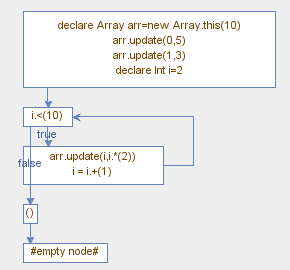
\includegraphics{cfg.png}
\caption{The CFG structure}
\label{fig:cfg}
\end{figure}

\begin{figure}
\centering
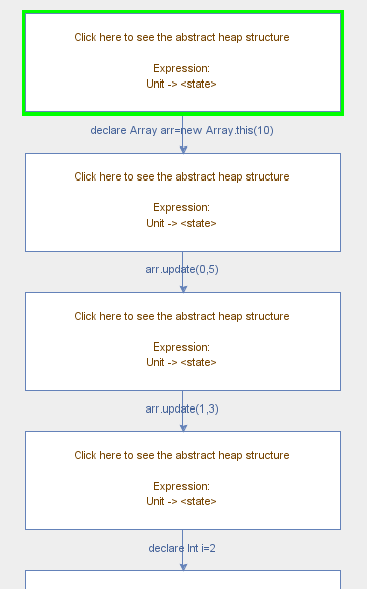
\includegraphics{block.png}
\caption{The block structure}
\label{fig:block}
\end{figure}

\begin{figure}
\centering
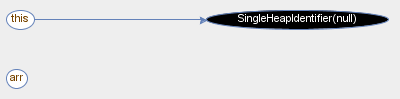
\includegraphics{heap.png}
\caption{The heap structure}
\label{fig:heap}
\end{figure}

\begin{figure}
\centering
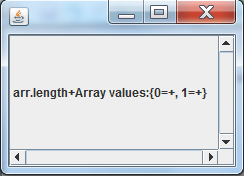
\includegraphics{node.png}
\caption{The string representation of a single node}
\label{fig:node}
\end{figure}

\section{How to run the analysis}
Unluckily, the last version of Scala compiler (2.8) has some problems when is called by Java code. The (quick) workaround I found is as follows:
\begin{itemize}
\item you can implement your analysis completely in Java
\item you compile your analysis and create a jar file
\item you put it on the Scala classpath
\item you launch the analysis through a Scala class that simply invokes the main method.
\end{itemize}
In the same way, you can create a Java project in Eclipse, and then a Scala project referencing the Java project in the Scala one. In this way, you can also put breakpoints on your Java code and debug the analysis launched through Scala.

The code of the Scala class that launches the analysis will look like the following one (where package \statement{AVPProject} contains the implementation of your analysis and \statement{YourAnalysis} is your implementation of the abstract class \statement{AVPProject}):

\begin{lstlisting}
import AVPProject._;
import ch.ethz.inf.pm.sample.userinterfaces._

object Run {
  def main(args : Array[String]) : Unit = {
	  ArrayAnalysis.analyze(
		"example1",
		"C:\\Users\\Pietro\\workspace\\Sample\\src\\Examples\\AVP2010.scala",
		new YourAnalysis()
	  );
  }
}
\end{lstlisting}

In order to compile and run the analysis you need also to put on the classpath some libraries (\statement{jgraphx.jar}, \statement{sample.jar}, \statement{scala-library.jar}, and \statement{scala-compiler.jar}). For the Scala project, you need only \statement{jgraphx.jar} and \statement{sample.jar}.

In addition, you need to install Scala (\texttt{http://www.scala-lang.org/downloads}), and, if you use Eclipse (\texttt{http://www.eclipse.org/}), the Scala plugin (\texttt{http://www.scala-ide.org/}).

\end{document}



